\begin{figure}[t]
 \centering
  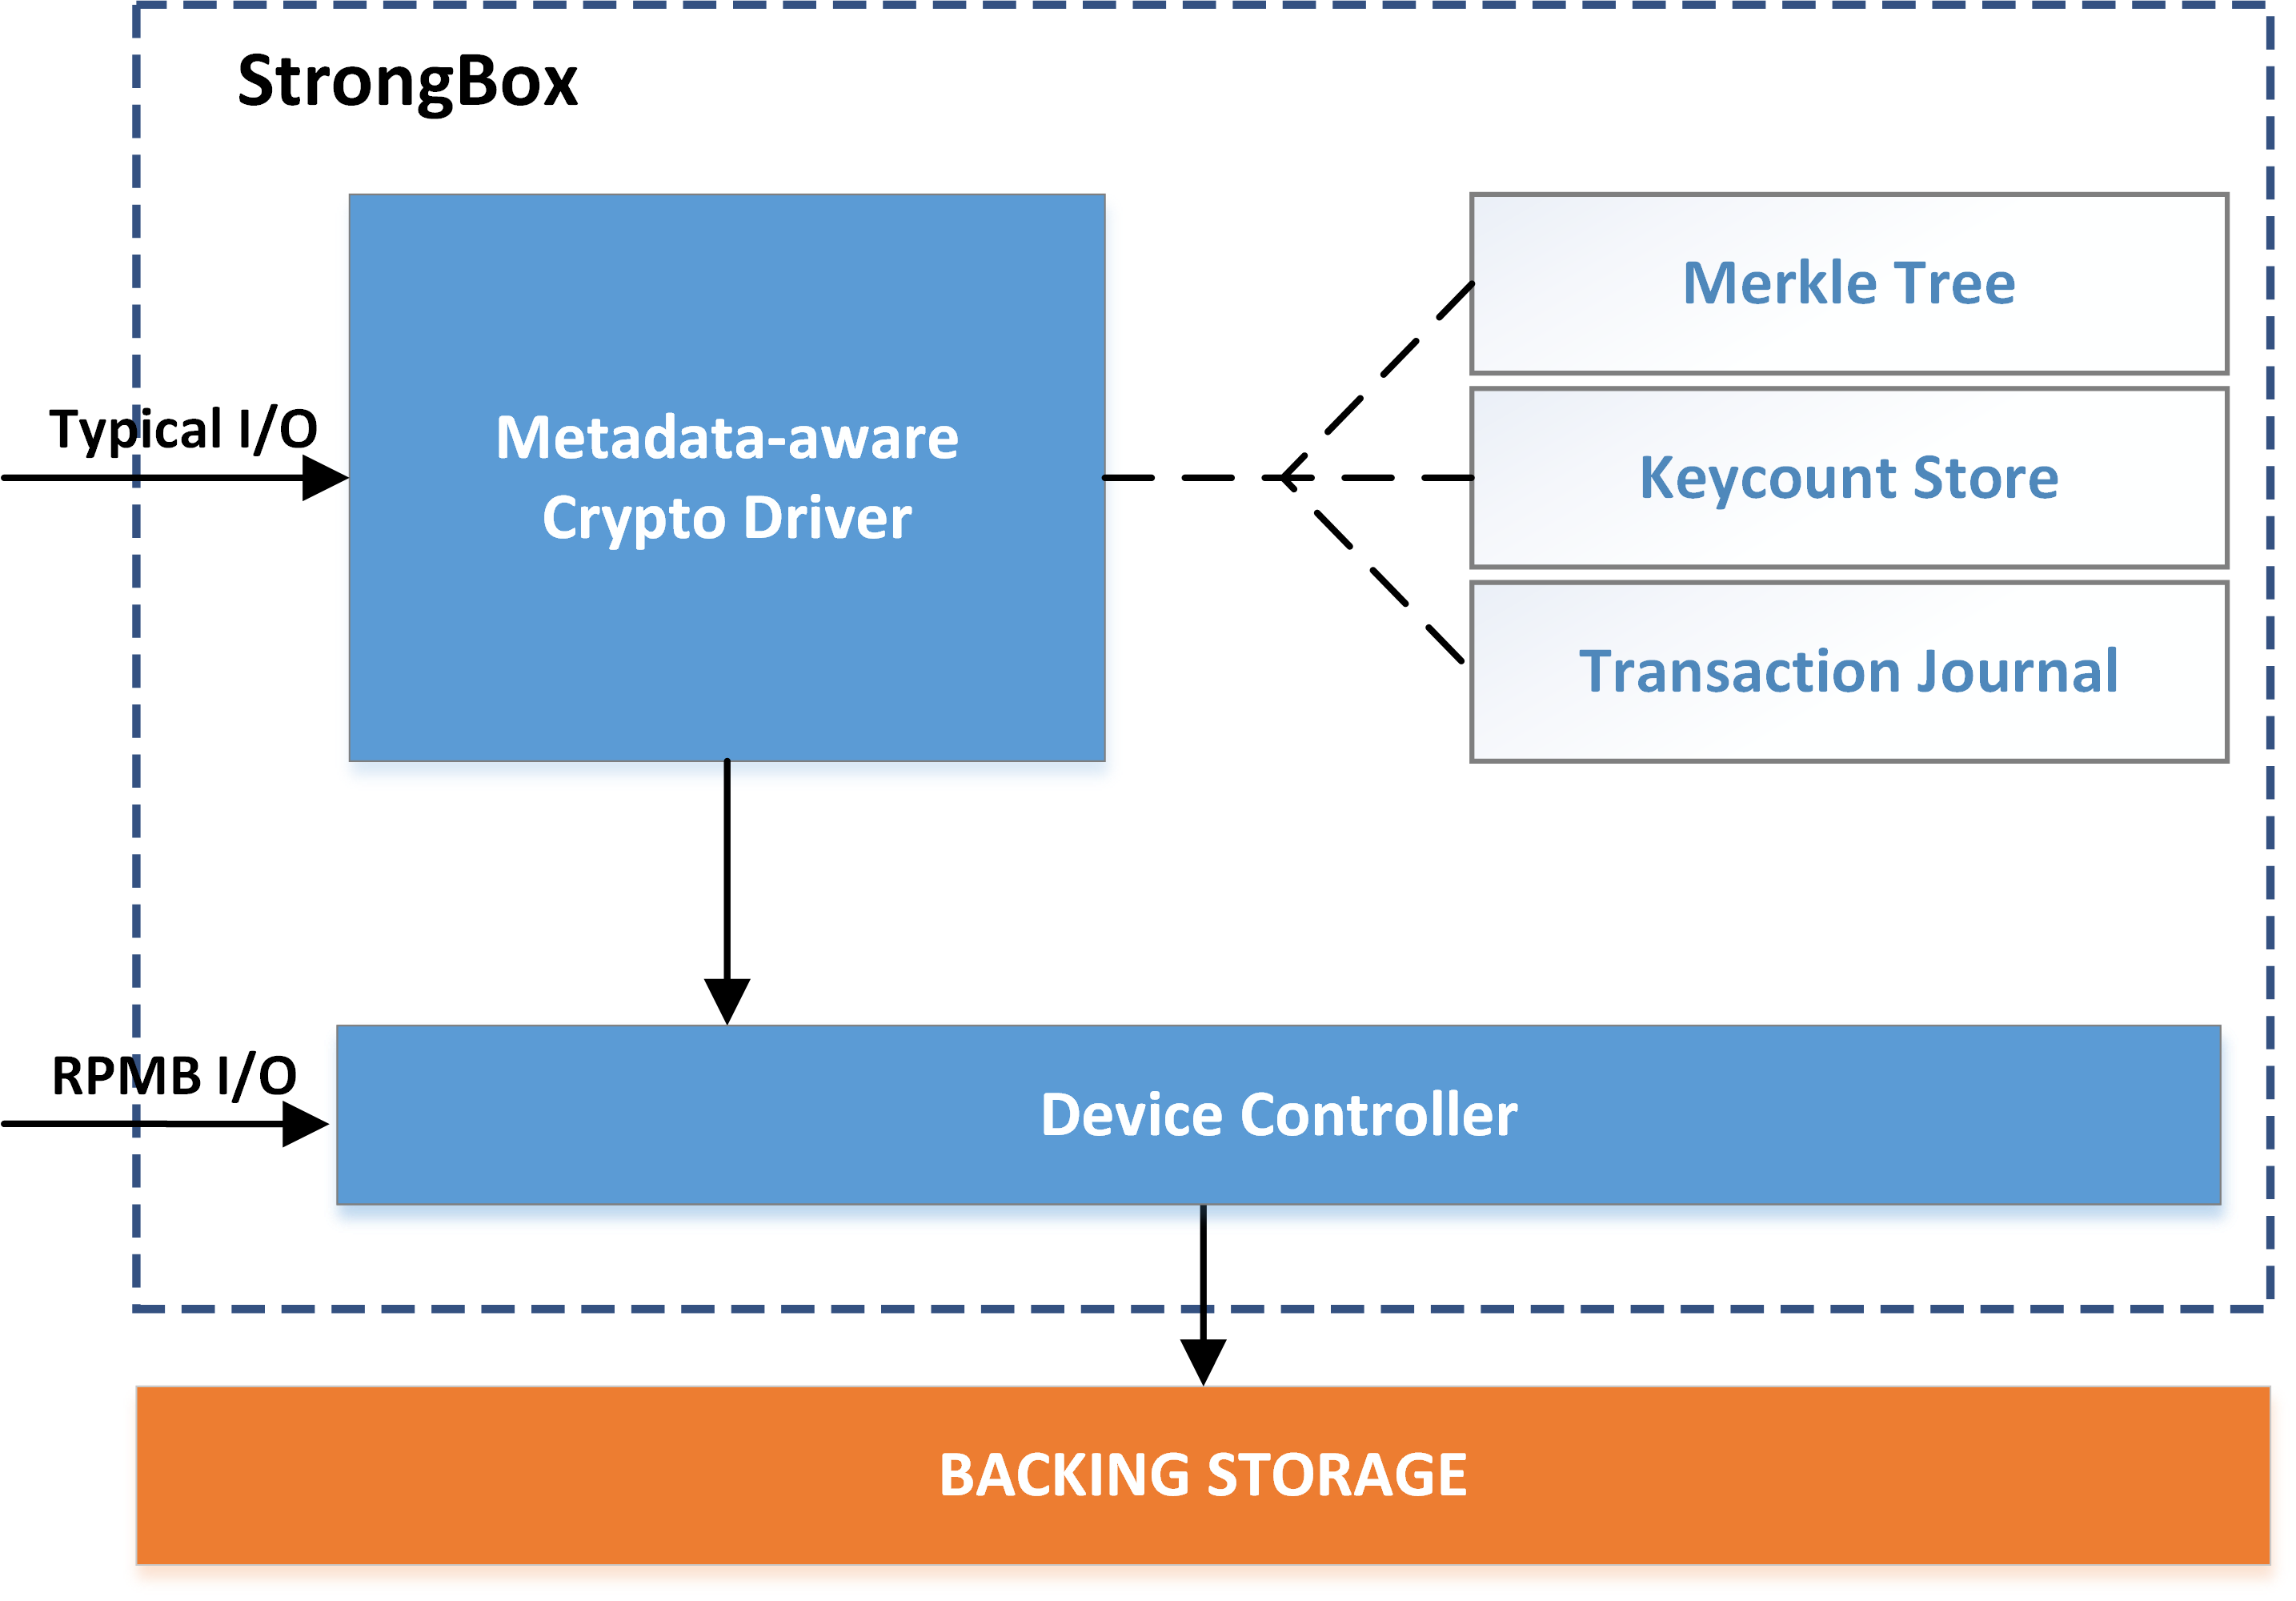
\includegraphics[width=\linewidth]{overview.png}
   \caption{Overview of the \SYSTEM{} construction.}\label{fig:overview}
\end{figure}

\section{\SYSTEM{} Design}\label{sec:design}

\TODO{Exactly how much of the original StrongBox should be explained here? Is
this too much? Too little?}

\SYSTEM{}, like StrongBox, is a translation layer positioned between the block
layer and the operating system's virtual file system~\cite{StrongBox}. There are
several places \SYSTEM{} could be implemented in the system stack: as part of an
actual kernel Log-structured File System (LFS) module like the F2FS filesystem,
as a block device or virtual block device in the manner of dm-crypt, or within a
device controller such as an SSD drive controller's FTL~\cite{StrongBox}.

\figref{overview} illustrates the \SYSTEM{} design. \SYSTEM{} manages five
metadata components: an in-memory \emph{Merkle Tree}; two drive-backed byte
arrays, \ie{the \emph{Keycount Store} and the \emph{Transaction Journal}}; a
globally persistent cryptographically secure monotonic counter; and a flexible
drive-backed store for per-nugget cipher-specific metadata. For our
monotonic counter implementation, we used a \emph{Replay Protected Memory Block}
(RPMB).

These five components are tightly integrated into the cryptographic driver,
which handles data encryption, decryption, overwrite detection, integrity
protection, and the application of cipher switching strategies. The
cryptographic driver interacts with 1) the overlying LFS through traditional I/O
passed through the Linux Virtual Filesystem Switch (VFS) as well as 2) the
underlying backing store through the device controller block I/O layer.

\begin{figure}[t]
 \centering
  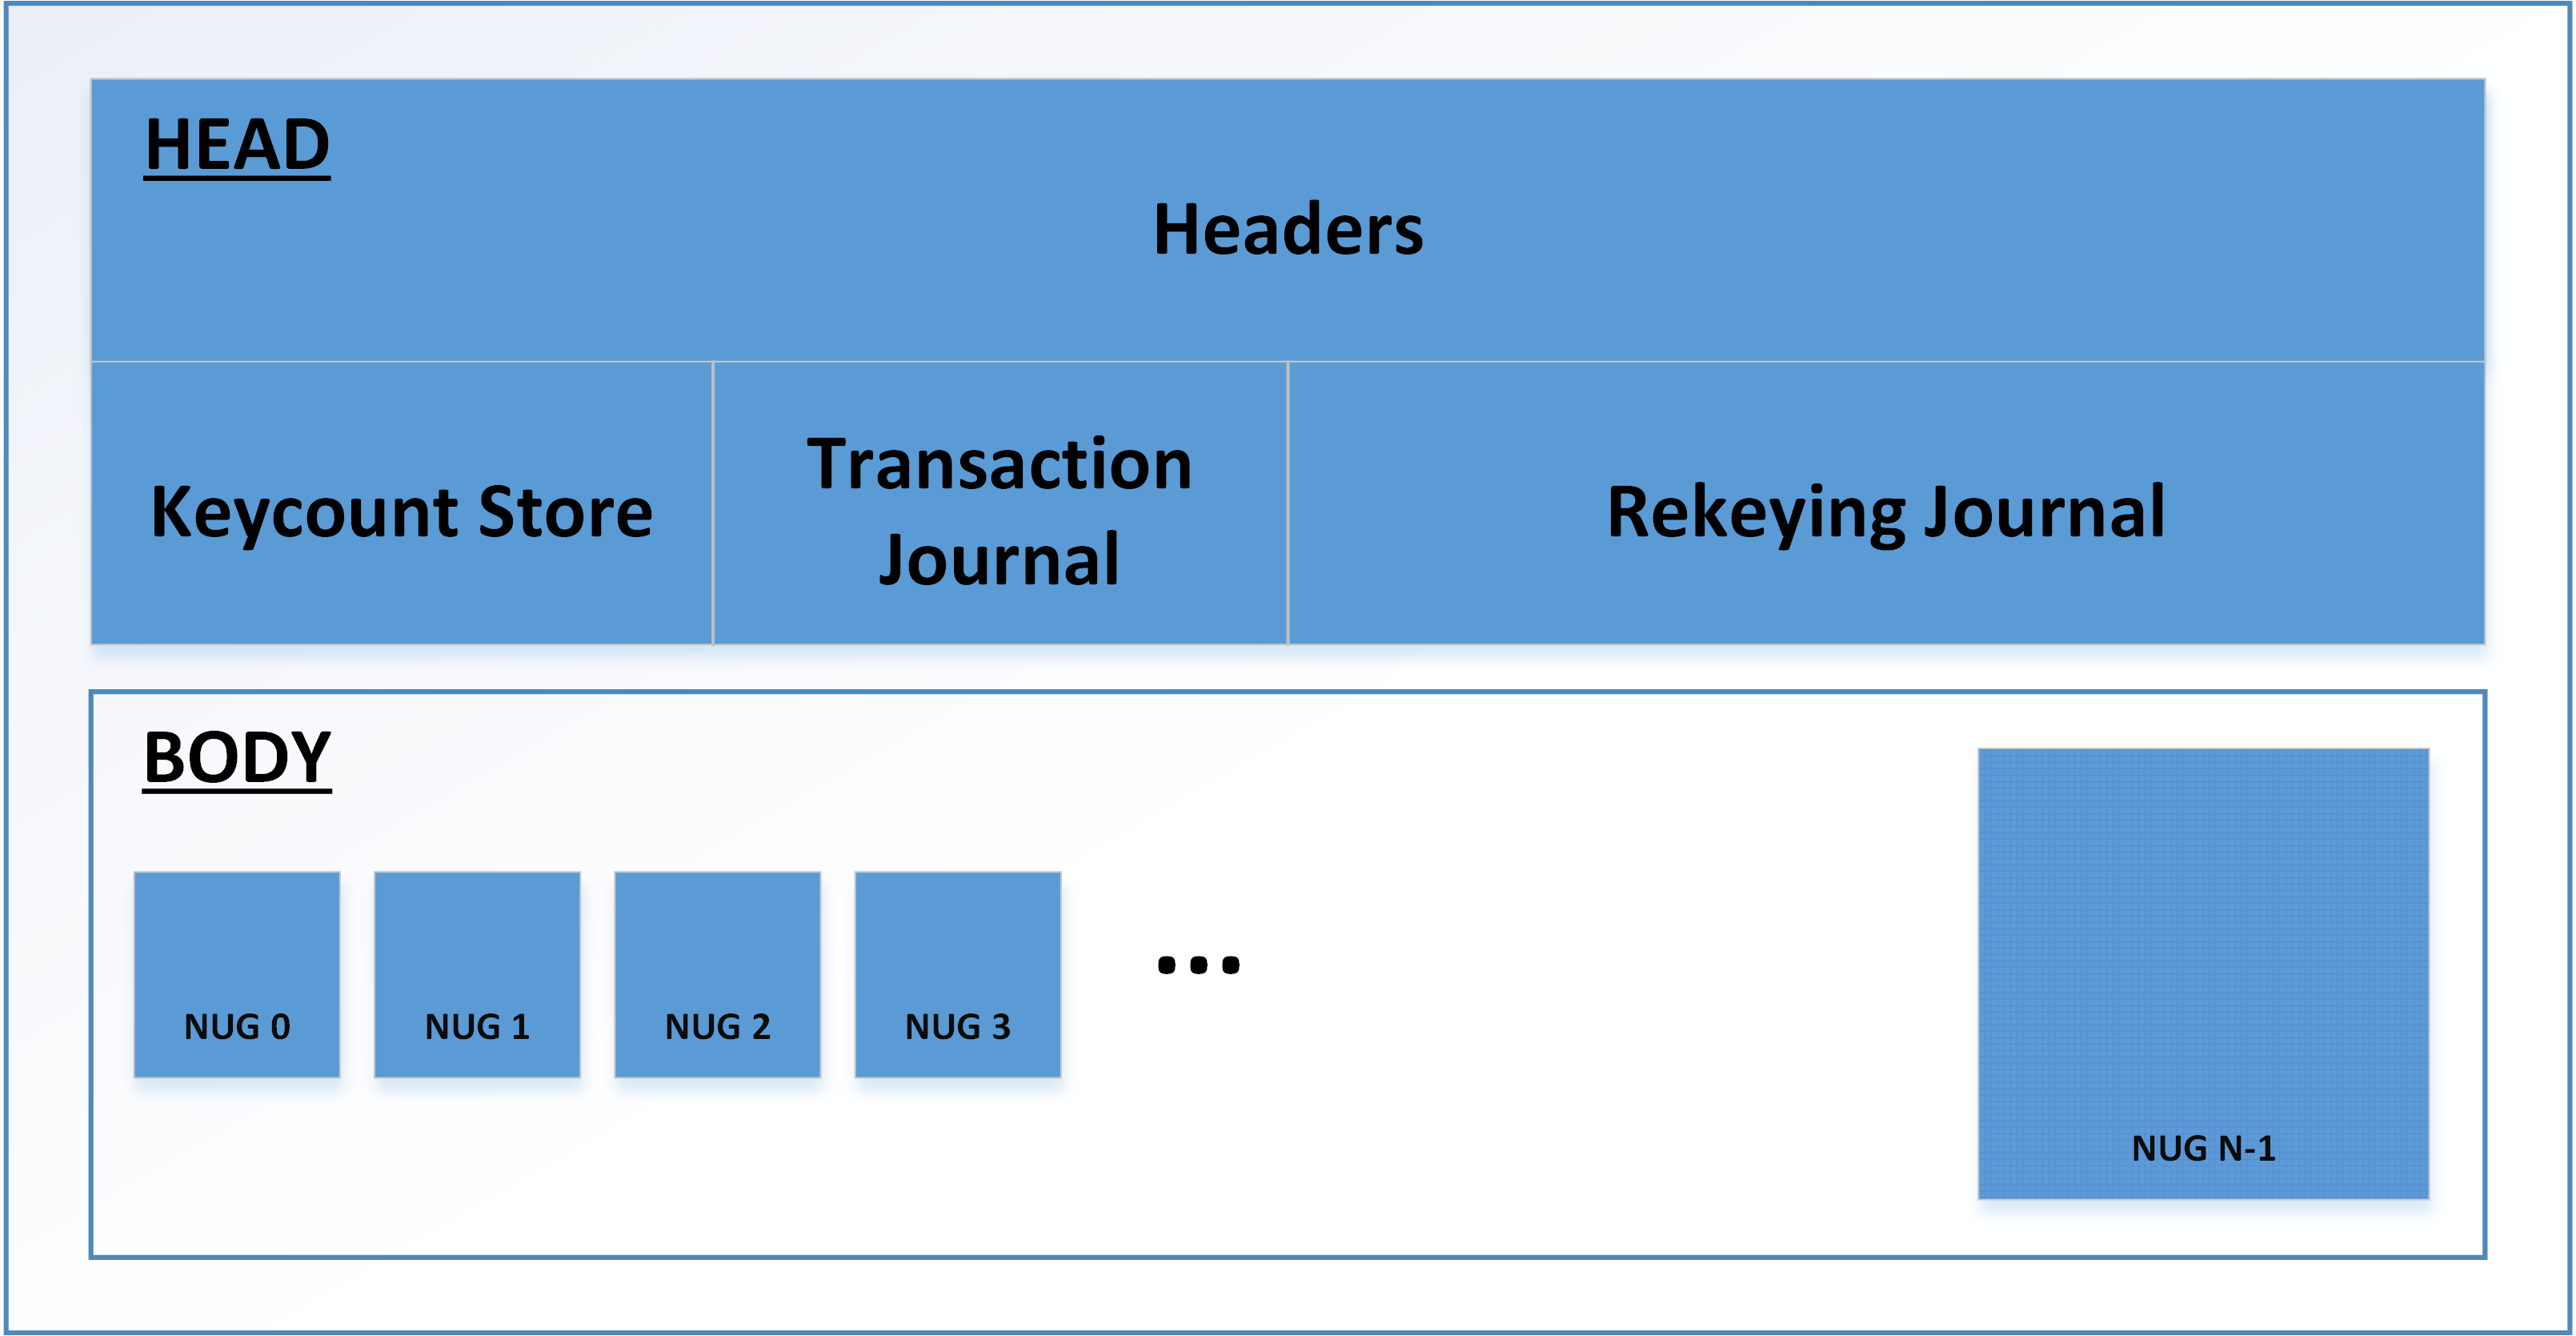
\includegraphics[width=\linewidth]{backstore.png}
   \caption{Layout of \SYSTEM{}'s backing storage.}\label{fig:backstore}
\end{figure}

\TODO{Backing store paragraph}

\TODO{Key insights and contributions paragraph (if necessary?)}

In the rest of this section, we describe our cipher switching strategies,
pluggable stream cipher API, and related design challenges with these
components. This is followed by an explanation of implementation-specific
details and a discussion of the overall implications and limitations of
\SYSTEM{}'s design.

\subsection{Cipher Switching Strategies}

\TODO{A sentence}

\subsubsection{Forward-Opportunistic}

\TODO{A paragraph}

\subsubsection{Forward-Immediate}

\TODO{A paragraph}

\subsubsection{Selective-Immediate}

\TODO{A paragraph}

\subsubsection{Mirrored-Immediate}

\TODO{A paragraph}

\subsection{Pluggable Stream Cipher API}

\TODO{Some paragraphs}

\subsection{Challenges}

\TODO{Performance overhead paragraph}

\TODO{Spatial overhead paragraph}

\subsection{Implementation}\label{sec:implementation}

Our \SYSTEM{} implementation consists of 9,491 lines of C code; our test suite
consists of 6,077 lines of C code. All together, our solution is comprised of
15,568 lines of C code. \SYSTEM{} uses OpenSSL version 1.1.0h and LibSodium
version 1.0.12 for its AES-XTS implementation. \TODO{Sentence or two about the
origin of estream cipher implementations}. As with the original StrongBox, the
Merkle Tree implementation is from the Secure Block Device~\cite{SBD}. \SYSTEM{}
implementation is publicly available open-source.\footnote{\SystemURI}.

For a fair comparison with the original StrongBox implementation, we mirror
their use of the BUSE~\cite{BUSE} virtual block device as our device controller.
BUSE is a thin (200 LoC) wrapper around the standard Linux Network Block Device
(NBD). Buse allows an operating system to transact block I/O requests to and
from virtual block devices exposed via domain socket.

\subsection{Discussion}

\TODO{Limitations.}
